\documentclass[]{jarticle}
\usepackage[dvipdfmx]{graphicx}
\usepackage{float}
\usepackage{subcaption}
\usepackage[dvipdfmx]{graphicx,xcolor}

\begin{document}
\title{$B8&5f?JD=Js9p(B}
\author{$B7W;;?@7P2J3X8&5f<<(B\\M2 $BB<>eFXI'(B}
\maketitle
 \section{$B8&5fGX7J(B}
 \section{$BJ}K!(B}
 $BK\8&5f$NJ}K!$O<g$K(BTorben-Nielsen et al\cite{torben2009systematic}$B$r;29M$K$7(B
 $B$F$$$k(B. $BJ}K!$N35N,$O(B, $B$"$i$+$8$a@_Dj$7$??@7P:YK&$N5!G=$r$&$^$/<B8=$9$k(B
 $B?@7P:YK&7ABV$r?J2=E*%"%k%4%j%:%`$rMQ$$$FC5:w$9$k$H$$$&$b$N$G$"$k(B. $B?@7P:YK&$N7A(B
 $BBV$O3NN(E*$KM?$($i$l(B, $B$=$N7ABV@8@.$N:]$KMQ$$$k%Q%i%a!<%?$r?J2=E*%"%k%4(B
 $B%j%:%`$K$*$1$k0dEA;R$H$9$k(B. $BJ}K!$N35N,?^$r0J2<$N?^(B\ref{inverse_approach}$B$K<($9(B. 

  %inverse approach$B$N35N,?^$r$N$;$k(B
 \begin{figure}[h]
  \centering
  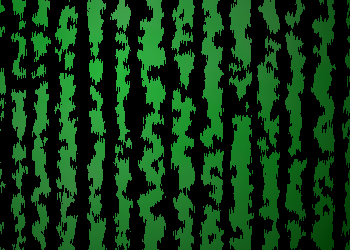
\includegraphics[width=5cm]{./Images/temp.png} 
  \caption{inverse approach}
  \label{inverse_approach}
 \end{figure}

 $B0J2<$N@a$K$*$$$F(B, $BJ}K!$N>\:Y(B($B7ABV@8@.(B, $B?J2=E*%"%k%4%j(B
 $B%:%`(B, $B%7%_%e%l!<%7%g%s(B)$B$r=R$Y$k(B. 

  \subsection{$B7ABV@8@.(B}
   \subsubsection{$B?@7P:YK&7ABV$NI=8=J}K!(B}
   %$B0l1~$3$l$K$b;29MJ88%$,$"$k(B?
   %L-system$B$r;H$C$F$$$k$H8@$C$?J}$,$h$$$+(B?
   $B?@7P:YK&$N7ABV$r7W;;5!>e$GI=8=$9$k$?$a$K(B, $B?@7P:YK&$N7ABV$O;0<!856u4V(B
   $B>e$KG[CV$5$l$?N)BN?^7A$N=89g$H$7$F07$&(B.$B0J2<$N?^(B
   \ref{reconstructed-neuron}$B$K:F8=$7$??@7P:YK&$NNc$r<($9(B. $BK\8&5f$G$O?@(B
   $B7P:YK&$N:YK&BN$*$h$S<y>uFM5/$N$_$rMQ$$$k$N$G(B, $B<4:w$K$D$$$F$O07$o$J$$(B. 
   
   \begin{figure}[h]
    \centering
    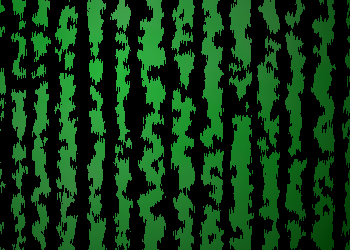
\includegraphics[width=5cm]{./Images/temp.png} 
    \caption{$B:F8=$5$l$??@7P:YK&$NNc(B}
  \label{reconstructed-neuron}
   \end{figure}
   
   $B?@7P:YK&$N:YK&BN$O5e$H$7$FI=8=$7(B, $B$=$NB>$N<y>uFM5/$O1_Cl$N=89g$H$7$F(B
   $BI=8=$9$k(B. $B:YK&BN$ND>7B$O(B$25{\mu}m$$B$H$7$?(B. $B<y>uFM5/$rI=$91_Cl$OKvC<It(B
   $BJ,$GB>$N1_Cl$d:YK&BN$H@\$7$F$*$j(B, $B$3$NItJ,$GB>$H7k9g$7$F$$$k$H$_$J$9(B.
   $B$=$NItJ,0J30$GJ#?t$N1_Cl$,6u4VE*$K=E$J$C$F$$$?$H$7$F$b$=$NItJ,$O7k9g(B
   $B$7$F$$$k$H$O$_$J$5$J$$(B. 

   $B:YK&BN$HD>@\7k9g$7$F$$$k1_Cl$r(BStem$B$H8F$S(B, $B$=$l0J30$N1_Cl$r(Bbranch$B$H8F(B
   $B$V(B. Stem$B$+$i?-$S$k0l$D$N<y>u9=B$$r(B, Stem$B$b4^$a$F0l$D$N<y>uFM5/$HDj5A$9$k(B. 
   $B$9$J$o$A?@7P:YK&$O$R$H$D$N:YK&BN$HJ#?t$N<y>uFM5/$r;}$D(B. $B$3$l$i$NDj5A$r?^(B
   \ref{reconstructed-neuron}$B$K<($9(B. 

   \begin{figure}[h]
    \centering
    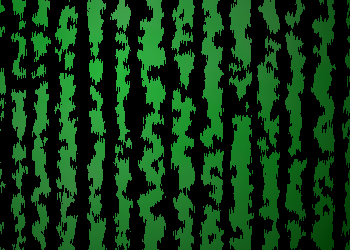
\includegraphics[width=5cm]{./Images/temp.png} 
    \caption{$B:YK&BN(B, Stem, $B<y>uFM5/$NNc(B}
  \label{mor-determination}
   \end{figure}

   $B?@7P:YK&7ABV$N@8@.$O(B, $B:G=i$K;0<!856u4V$N86E@$K:YK&BN$rG[CV$7$=$l$K8D!9(B
   $B$N<y>uFM5/$r3NN(E*$K@8@.$9$k$3$H$G9T$&(B.$B0J2<$GC10l<y>uFM5/$N@8@.J}K!$r(B
   $B=R$Y$k(B. 
   \subsubsection{$BC10l<y>uFM5/7ABV$N@8@.J}K!(B}
   %$B%"%k%4%j%:%_%C%/$K=q$/(B
   $B<y>uFM5/$N@8@.J}K!$O4pK\E*$K(BDOL-system\cite{prusinkiewicz1990}$B$N<jK!(B
   $B$r4p$K$7$F$$$k(B. DOL-System$B$O$"$k5-9f$N=89g$H(B, $B$=$N5-9f$NCV$-49$(5,B'(B
   $B$N=89g$+$i$J$k(B. 

   $B$R$H$D$N<y>uFM5/$O0J2<$NI=(B\ref{tree_param}$B$KI=$5$l$k%Q%i%a!<%?%;%C%H(B
   $B$r;}$D(B.$B$3$N%Q%i%a!<%?%;%C%H$rMQ$$$F3NN(E*$K<y>uFM5/$,@8@.$5$l$k(B. $B$^$?(B
   $B$3$N%Q%i%a!<%?%;%C%H$O8e$K=R$Y$k?J2=E*%"%k%4%j%:%`$N0dEA;R$G$b$"$k(B. 

   \begin{table}[h]
    \caption{$B<y>uFM5/%Q%i%a!<%?%;%C%H(B}
    \label{tree_param}
    \begin{center}
     \begin{tabular}[t]{|c|c|} \hline
      $B%Q%i%a!<%?L>(B & $B@bL@(B \\ \hline \hline
      Stem elevation MIEW & Stem$B$N6D3Q7hDj$KMQ$$$kJ?6QCM(B \\ \hline
      Stem elevation SIGMA & Stem$B$N6D3Q7hDj$KMQ$$$kI8=`JP:9CM(B  \\ \hline
      Stem rotation MIEW  & Stem$B$N2sE>3Q7hDj$KMQ$$$kJ?6QCM(B \\ \hline
      Stem rotation SIGMA  & Stem$B$N2sE>3Q7hDj$KMQ$$$kI8=`JP:9CM(B \\ \hline
      Stem diameter  & Stem$B$ND>7B(B \\ \hline
      Segment length  & Stem$B$*$h$S(Bbranch$B$ND9$5(B \\ \hline
      Branch elevation MIEW & branch$B$N6D3Q7hDj$KMQ$$$kJ?6QCM(B \\ \hline
      Branch elevation SIGMA & branch$B$N6D3Q7hDj$KMQ$$$kI8=`JP:9CM(B \\ \hline
      Branch rotation MIEW  & branch$B$N2sE>3Q7hDj$KMQ$$$kJ?6QCM(B \\ \hline
      Branch rotation SIGMA  & branch$B$N2sE>3Q7hDj$KMQ$$$kI8=`JP:9CM(B  \\ \hline
      Bifurcation $\alpha$ & $B<y>u9=B$$NJ,4tF3F~H=Dj$KMQ$$$k(B$alpha$$BCM(B \\ \hline
      Bifurcation $\beta$  & $B<y>u9=B$$NJ,4tF3F~H=Dj$KMQ$$$k(B$beta$$BCM(B \\ \hline
      Termination $\alpha$ & $B<y>u9=B$$N=*C<E@F3F~H=Dj$KMQ$$$k(B$alpha$$BCM(B \\ \hline
      Termination $\beta$  & $B<y>u9=B$$N=*C<E@F3F~H=Dj$KMQ$$$k(B$beta$$BCM(B \\ \hline
      K Stem conductance & Stem$B$N(BKa$B%3%s%@%/%?%s%9CM(B \\ \hline
      K taper rate  & Ka$B%3%s%@%/%?%s%9$NEAHBN((B \\ \hline
      Ca Stem conductance & Stem$B$N(BCaT$B%3%s%@%/%?%s%9CM(B \\ \hline
      Ca taper rate  & CaT$B%3%s%@%/%?%s%9$NEAHBN((B \\ \hline
     \end{tabular}
    \end{center}
   \end{table}

   $B<y>uFM5/7ABV@8@.$N%"%k%4%j%:%`$r0J2<$N?^(B\ref{Dendrite-argorythm}$B$K<($9(B.

   \begin{figure}[h]
    \centering
    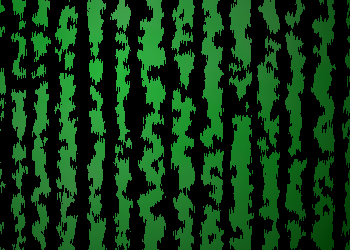
\includegraphics[width=5cm]{./Images/temp.png} 
    \caption{$B<y>uFM5/7ABV@8@.%"%k%4%j%:%`(B}
  \label{Dendrite-argorythm}
   \end{figure}

   \begin{enumerate}
    \item \textbf{$B:YK&BN$NG[CV(B}\\
	  $B;0<!856u4V$N86E@$K:YK&BN$rG[CV$9$k(B
    \item \textbf{Stem$B$N@8@.(B}\\
	  $B0J2<$NI=(B\ref{stem_param}$B$K<($5$l$k7ABV%Q%i%a!<%?$r7hDj$9$k$3$H(B
	  $B$G(BStem$B$r@8@.$9$k(B. 
	  \begin{table}[h]
	   \caption{Stem$B@8@.(B}
	   \label{stem_param}
	   \begin{center}
	    \begin{tabular}[t]{|c|c|c|c|} \hline
	     $B%Q%i%a!<%?L>(B & $B@bL@(B & $B3NN(J,I[(B & $B3NN(%Q%i%a!<%?(B($B0dEA;R(B) \\ \hline
	     \hline
	     length & $BD9$5(B & Constant & Segment length \\ \hline
	     elevation & $B6D3Q(B & Gausian & Stem elevation MIEW, Stem elevation SIGMA \\ \hline
	     rotation  & $B2sE>3Q(B & Gausian & Stem rotation MIEW, Stem rotation
			 SIGMA \\ \hline
	    \end{tabular}
	   \end{center}
	  \end{table}
   \end{enumerate}
   %$B6D3Q!"2sE>3Q$K$D$$$F$N@bL@$r$$$l$k(B
  \subsection{$B?J2=E*%"%k%4%j%:%`(B}
   \subsubsection{$B0lE@8r:5(B}
   \subsubsection{$BFMA3JQ0[(B}
  \subsection{$B%7%_%e%l!<%7%g%s(B}
 \section{$B7k2L(B}
 \section{$B9M;!(B}
 \bibliographystyle{jplain}
 \bibliography{biblio}
\end{document}